\documentclass{ctexart}
\usepackage{Note}
\usepackage{makecell}
\setCJKmainfont[
  BoldFont = 思源宋体 Bold,
  ItalicFont = 楷体,
]{宋体}
\author{2400011785 蒋锦豪}
\title{\tbf{结构化学\ 第6章作业}}
\begin{document}
\maketitle
\begin{homework}[1.]
    填写附表1.
\end{homework}
\begin{solution}
如下表所示.
\begin{table}[H]\centering
    \begin{tabular}{|c|c|c|c|c|c|c|}\hline
        & \ce{Cu} & \ce{Na} & \ce{CsCl} & \ce{C}(金刚石) & \ce{C}(石墨) & \ce{Mg} \\\hline
        结构基元组成 & $1\ce{Cu}$ & $1\ce{Na}$ & $1\ce{CsCl}$ & $2\ce{C}$ & $4\ce{C}$ & $2\ce{Mg}$ \\\hline
        特征对称元素 & $4C_3$ & $4C_3$ & $4C_3$ & $4C_3$ & $6_3$ & $6_3$ \\\hline
        晶系 & 立方晶系 & 立方晶系 & 立方晶系 & 立方晶系 & 六方晶系 & 六方晶系 \\\hline
        晶胞中的结构基元数 & $4$ & $2$ & $1$ & $4$ & $1$ & $1$ \\\hline
        点阵型式 & $\text{cF}$ & $\text{cI}$ & $\text{cP}$ & $\text{cF}$ & $\text{hP}$ & $\text{hP}$ \\\hline
        原子坐标 & \makecell[c]{
            $(0,0,0)$\\
            $(0,\frac12,\frac12)$\\
            $(\frac12,0,\frac12)$\\
            $(\frac12,\frac12,0)$
        } & \makecell[c]{
            $(0,0,0)$\\
            $(\frac12,\frac12,\frac12)$
        } & \makecell[c]{
            \ce{Cl}\,$(0,0,0)$\\
            \ce{Cs}\,$(\frac12,\frac12,\frac12)$
        } & \makecell[c]{
            $(0,0,0)$\\
            $(0,\frac12,\frac12)$\\
            $(\frac12,0,\frac12)$\\
            $(\frac12,\frac12,0)$\\
            $(\frac14,\frac34,\frac14)$\\
            $(\frac34,\frac14,\frac14)$\\
            $(\frac14,\frac14,\frac34)$\\
            $(\frac34,\frac34,\frac34)$
        } & \makecell[c]{
            $(0,0,0)$\\
            $(\frac23,\frac13,0)$\\
            $(0,0,\frac12)$\\
            $(\frac13,\frac23,\frac12)$
        } & \makecell[c]{
            $(0,0,0)$\\
            $(\frac13,\frac23,\frac12)$
        } \\\hline
    \end{tabular}
\end{table}
\end{solution}
\begin{homework}[2.]
    作图表明微观对称元素.
    \begin{enumerate}[label=\tbf{(\alph*)}]
        \item 金刚石空间群的国际符号为$\text{F}\,4_1/\text{d}\,\bar{3}\,2/\text{m}$,简记为$\text{F}\,\text{d}\,\bar{3}\,\text{m}$,熊夫利记号为$O_{\text{h}}^7$.试画出金刚石晶胞结构投影图,在图上用微观对称元素记号标出一个$\text{d}$滑移面以及$4_1$, $4_3$螺旋轴.
        \item 画出金属镁晶胞沿六重轴方向的结构投影图，并在图上标出六重轴($\bar{6}$和$6_3$)的位置.
        \item 对石墨重复\tbf{(b)}中操作.
    \end{enumerate}
\end{homework}
\begin{solution}
    如下图所示.
    \begin{figure}[H]\centering
        \begin{subfigure}[b]{.3\linewidth}\centering
            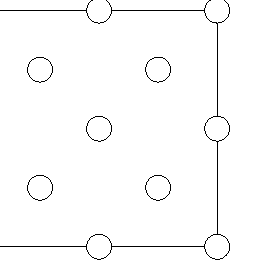
\includegraphics[scale=0.3]{figure/2(a).png}
            \caption{金刚石}
        \end{subfigure}
        \begin{subfigure}[b]{.3\linewidth}\centering
            \input{figure/2(b).tex}
            \caption{镁}
        \end{subfigure}
        \begin{subfigure}[b]{.3\linewidth}\centering
            \documentclass{standalone}
\usepackage{Note}
\begin{document}
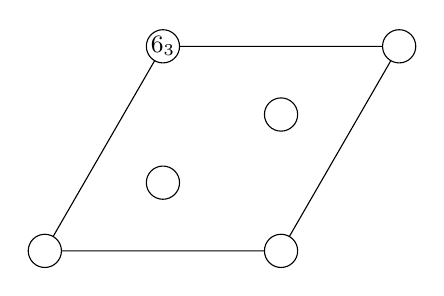
\begin{tikzpicture}[scale=0.75]
    \draw[-] (0,0) -- (4,0) -- (6,3.464) -- (2,3.464) -- (0,0);
    \filldraw[fill=white, draw=black] (0,0) circle (8pt);
    \filldraw[fill=white, draw=black] (4,0) circle (8pt);
    \filldraw[fill=white, draw=black] (6,3.464) circle (8pt);
    \filldraw[fill=white, draw=black] (2,3.464) circle (8pt);
    \filldraw[fill=white, draw=black] (4,2.309) circle (8pt);
    \filldraw[fill=white, draw=black] (2,1.155) circle (8pt);
    \node at (2,3.464) {\small$6_3$};
\end{tikzpicture}
\end{document}
            \caption{石墨}
        \end{subfigure}
    \end{figure}
\end{solution}
\begin{homework}[3.]
    指出下图中置于立方晶格中的红色多面体各个面的晶面指标.
\end{homework}
\begin{solution}
如下图所示.
\begin{figure}[H]\centering
    \begin{subfigure}[b]{0.24\linewidth}\centering
        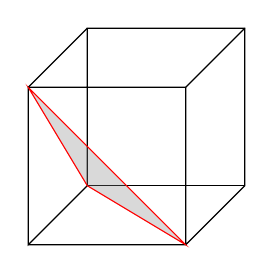
\begin{tikzpicture}[scale=0.5]
            \draw[-] (0,0) -- (4,0) -- (4,4) -- (0,4) -- (0,0) -- (1.5,1.5) -- (1.5,5.5) -- (5.5,5.5) -- (5.5,1.5) -- (4,0);
            \draw[-] (4,4) -- (5.5,5.5);
            \draw[-] (0,4) -- (1.5,5.5);
            \draw[-] (1.5,1.5) -- (5.5,1.5);
            \filldraw[
                fill = gray,
                fill opacity = 0.3,
                draw = red
            ]
            (1.5,1.5) -- (0,4) --(4,0) --cycle;
        \end{tikzpicture}
        \caption{$\bar{1}11$}
    \end{subfigure}
    \begin{subfigure}[b]{0.24\linewidth}\centering
        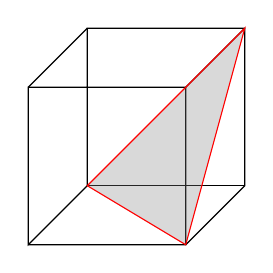
\begin{tikzpicture}[scale=0.5]
            \draw[-] (0,0) -- (4,0) -- (4,4) -- (0,4) -- (0,0) -- (1.5,1.5) -- (1.5,5.5) -- (5.5,5.5) -- (5.5,1.5) -- (4,0);
            \draw[-] (4,4) -- (5.5,5.5);
            \draw[-] (0,4) -- (1.5,5.5);
            \draw[-] (1.5,1.5) -- (5.5,1.5);
            \filldraw[
                fill = gray,
                fill opacity = 0.3,
                draw = red
            ]
            (1.5,1.5) -- (5.5,5.5) --(4,0) --cycle;
        \end{tikzpicture}
        \caption{$\bar{1}\bar{1}1$}
    \end{subfigure}
    \begin{subfigure}[b]{0.24\linewidth}\centering
        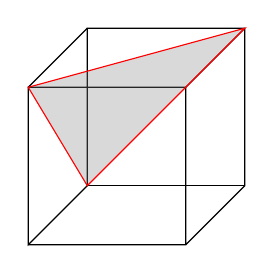
\begin{tikzpicture}[scale=0.5]
            \draw[-] (0,0) -- (4,0) -- (4,4) -- (0,4) -- (0,0) -- (1.5,1.5) -- (1.5,5.5) -- (5.5,5.5) -- (5.5,1.5) -- (4,0);
            \draw[-] (4,4) -- (5.5,5.5);
            \draw[-] (0,4) -- (1.5,5.5);
            \draw[-] (1.5,1.5) -- (5.5,1.5);
            \filldraw[
                fill = gray,
                fill opacity = 0.3,
                draw = red
            ]
            (1.5,1.5) -- (5.5,5.5) --(0,4) --cycle;
        \end{tikzpicture}
        \caption{$11\bar{1}$}
    \end{subfigure}
    \begin{subfigure}[b]{0.24\linewidth}\centering
        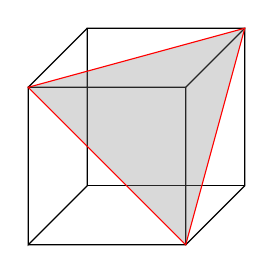
\begin{tikzpicture}[scale=0.5]
            \draw[-] (0,0) -- (4,0) -- (4,4) -- (0,4) -- (0,0) -- (1.5,1.5) -- (1.5,5.5) -- (5.5,5.5) -- (5.5,1.5) -- (4,0);
            \draw[-] (4,4) -- (5.5,5.5);
            \draw[-] (0,4) -- (1.5,5.5);
            \draw[-] (1.5,1.5) -- (5.5,1.5);
            \filldraw[
                fill = gray,
                fill opacity = 0.3,
                draw = red
            ]
            (0,4) -- (5.5,5.5) --(4,0) --cycle;
        \end{tikzpicture}
        \caption{$111$}
    \end{subfigure}
    \caption{正四面体}
\end{figure}
\begin{figure}[H]\centering
    \begin{subfigure}[b]{0.24\linewidth}\centering
        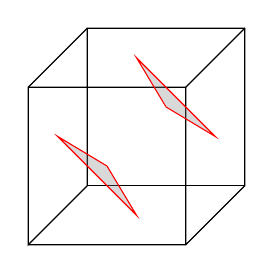
\begin{tikzpicture}[scale=0.5]
            \draw[-] (0,0) -- (4,0) -- (4,4) -- (0,4) -- (0,0) -- (1.5,1.5) -- (1.5,5.5) -- (5.5,5.5) -- (5.5,1.5) -- (4,0);
            \draw[-] (4,4) -- (5.5,5.5);
            \draw[-] (0,4) -- (1.5,5.5);
            \draw[-] (1.5,1.5) -- (5.5,1.5);
            \filldraw[
                fill = gray,
                fill opacity = 0.3,
                draw = red
            ]
            (0.75,2.75) -- (2,2) --(2.75,0.75) --cycle;
            \filldraw[
                fill = gray,
                fill opacity = 0.3,
                draw = red
            ](4.75,2.75) -- (3.5,3.5) --(2.75,4.75) --cycle;
        \end{tikzpicture}
        \caption{$\bar{1}11$}
    \end{subfigure}
    \begin{subfigure}[b]{0.24\linewidth}\centering
        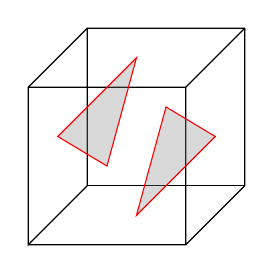
\begin{tikzpicture}[scale=0.5]
            \draw[-] (0,0) -- (4,0) -- (4,4) -- (0,4) -- (0,0) -- (1.5,1.5) -- (1.5,5.5) -- (5.5,5.5) -- (5.5,1.5) -- (4,0);
            \draw[-] (4,4) -- (5.5,5.5);
            \draw[-] (0,4) -- (1.5,5.5);
            \draw[-] (1.5,1.5) -- (5.5,1.5);
            \filldraw[
                fill = gray,
                fill opacity = 0.3,
                draw = red
            ]
            (0.75,2.75) -- (2,2) --(2.75,4.75) --cycle;
            \filldraw[
                fill = gray,
                fill opacity = 0.3,
                draw = red
            ]
            (4.75,2.75) -- (3.5,3.5) --(2.75,0.75) --cycle;
        \end{tikzpicture}
        \caption{$\bar{1}\bar{1}1$}
    \end{subfigure}
    \begin{subfigure}[b]{0.24\linewidth}\centering
        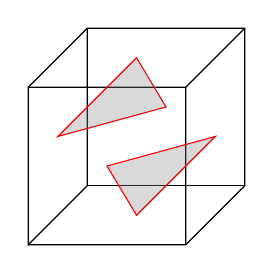
\begin{tikzpicture}[scale=0.5]
            \draw[-] (0,0) -- (4,0) -- (4,4) -- (0,4) -- (0,0) -- (1.5,1.5) -- (1.5,5.5) -- (5.5,5.5) -- (5.5,1.5) -- (4,0);
            \draw[-] (4,4) -- (5.5,5.5);
            \draw[-] (0,4) -- (1.5,5.5);
            \draw[-] (1.5,1.5) -- (5.5,1.5);
            \filldraw[
                fill = gray,
                fill opacity = 0.3,
                draw = red
            ]
            (0.75,2.75) -- (3.5,3.5) --(2.75,4.75) --cycle;
            \filldraw[
                fill = gray,
                fill opacity = 0.3,
                draw = red
            ]
            (4.75,2.75) -- (2,2) --(2.75,0.75) --cycle;
        \end{tikzpicture}
        \caption{$11\bar{1}$}
    \end{subfigure}
    \begin{subfigure}[b]{0.24\linewidth}\centering
        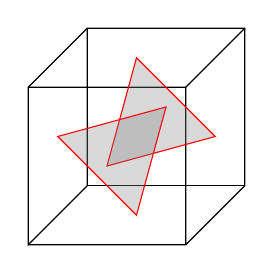
\begin{tikzpicture}[scale=0.5]
            \draw[-] (0,0) -- (4,0) -- (4,4) -- (0,4) -- (0,0) -- (1.5,1.5) -- (1.5,5.5) -- (5.5,5.5) -- (5.5,1.5) -- (4,0);
            \draw[-] (4,4) -- (5.5,5.5);
            \draw[-] (0,4) -- (1.5,5.5);
            \draw[-] (1.5,1.5) -- (5.5,1.5);
            \filldraw[
                fill = gray,
                fill opacity = 0.3,
                draw = red
            ]
            (4.75,2.75) -- (2,2) --(2.75,4.75) --cycle;
            \filldraw[
                fill = gray,
                fill opacity = 0.3,
                draw = red
            ]
            (0.75,2.75) -- (3.5,3.5) --(2.75,0.75) --cycle;
        \end{tikzpicture}
        \caption{$111$}
    \end{subfigure}
    \caption{正八面体}
\end{figure}
\begin{figure}[H]\centering
    \begin{subfigure}[b]{0.24\linewidth}\centering
        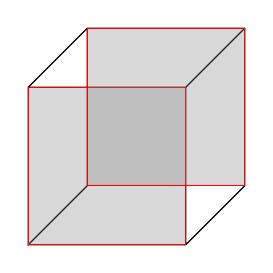
\begin{tikzpicture}[scale=0.5]
            \draw[-] (0,0) -- (4,0) -- (4,4) -- (0,4) -- (0,0) -- (1.5,1.5) -- (1.5,5.5) -- (5.5,5.5) -- (5.5,1.5) -- (4,0);
            \draw[-] (4,4) -- (5.5,5.5);
            \draw[-] (0,4) -- (1.5,5.5);
            \draw[-] (1.5,1.5) -- (5.5,1.5);
            \filldraw[
                fill = gray,
                fill opacity = 0.3,
                draw = red
            ]
            (0,0) -- (0,4) --(4,4) -- (4,0) --cycle;
            \filldraw[
                fill = gray,
                fill opacity = 0.3,
                draw = red
            ](1.5,1.5) -- (5.5,1.5) --(5.5,5.5) -- (1.5,5.5) --cycle;
        \end{tikzpicture}
        \caption{$010$}
    \end{subfigure}
    \begin{subfigure}[b]{0.24\linewidth}\centering
        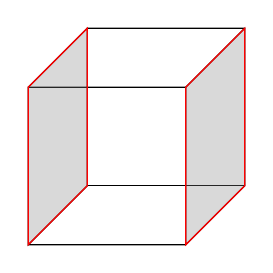
\begin{tikzpicture}[scale=0.5]
            \draw[-] (0,0) -- (4,0) -- (4,4) -- (0,4) -- (0,0) -- (1.5,1.5) -- (1.5,5.5) -- (5.5,5.5) -- (5.5,1.5) -- (4,0);
            \draw[-] (4,4) -- (5.5,5.5);
            \draw[-] (0,4) -- (1.5,5.5);
            \draw[-] (1.5,1.5) -- (5.5,1.5);
            \filldraw[
                fill = gray,
                fill opacity = 0.3,
                draw = red
            ]
            (0,0) -- (1.5,1.5) -- (1.5,5.5) -- (0,4) --cycle;
            \filldraw[
                fill = gray,
                fill opacity = 0.3,
                draw = red
            ]
            (4,0) -- (5.5,1.5) -- (5.5,5.5) -- (4,4) --cycle;
        \end{tikzpicture}
        \caption{$100$}
    \end{subfigure}
    \begin{subfigure}[b]{0.24\linewidth}\centering
        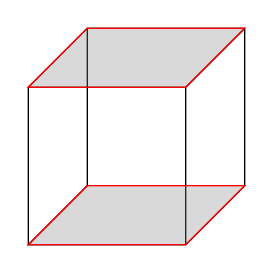
\begin{tikzpicture}[scale=0.5]
            \draw[-] (0,0) -- (4,0) -- (4,4) -- (0,4) -- (0,0) -- (1.5,1.5) -- (1.5,5.5) -- (5.5,5.5) -- (5.5,1.5) -- (4,0);
            \draw[-] (4,4) -- (5.5,5.5);
            \draw[-] (0,4) -- (1.5,5.5);
            \draw[-] (1.5,1.5) -- (5.5,1.5);
            \filldraw[
                fill = gray,
                fill opacity = 0.3,
                draw = red
            ]
            (0,0) -- (1.5,1.5) -- (5.5,1.5) -- (4,0) --cycle;
            \filldraw[
                fill = gray,
                fill opacity = 0.3,
                draw = red
            ]
            (0,4) -- (1.5,5.5) -- (5.5,5.5) -- (4,4) --cycle;
        \end{tikzpicture}
        \caption{$001$}
    \end{subfigure}
    \caption{正方体}
\end{figure}
\end{solution}
\begin{homework}[4.]
    填写附表2.
\end{homework}
\begin{solution}
如下表所示.在考虑半径比时,假定阳离子半径小于阴离子半径.
\begin{table}[H]\centering
    \begin{tabular}{|c|c|c|c|c|}\hline
        晶体 & \ce{NaCl} & \ce{CsCl} & 立方~\ce{ZnS} & 六方~\ce{ZnS} \\\hline
        负离子堆积方式 & 立方最密堆积 & 简单立方堆积 & 立方最密堆积 & 六方最密堆积 \\\hline
        \makecell[c]{正负离子半径比\\$r_+/r_-$} & $\left(\sqrt{2}-1,\sqrt{3}-1\right)$ & $\left(\sqrt{3}-1,1\right)$ & $\left(0,\sqrt{2}-1\right)$ & $\left(0,\sqrt{2}-1\right)$ \\\hline
        正负离子数量比 & $1:1$ & $1:1$ & $1:1$ & $1:1$ \\\hline
        正离子占据空隙 & 八面体空隙 & 立方体空隙 & 四面体空隙 & 四面体空隙 \\\hline
        正离子填隙率 & $100\%$ & $100\%$ & $50\%$ & $50\%$ \\\hline
        正离子配位数 & $6$ & $8$ & $4$ & $4$ \\\hline
        \makecell[c]{配位多面体\\连接方式} & 共棱连接 & 共面连接 & 共顶点连接 & 共顶点连接 \\\hline
        负离子配位数 & $6$ & $8$ & $4$ & $4$ \\\hline
        点阵型式 & cF & cP & cF & hP \\\hline
        结构基元 & $1\ce{NaCl}$ & $1\ce{CsCl}$ & $1\ce{ZnS}$ & $2\ce{ZnS}$ \\\hline
        晶胞内正负离子数 & $4$, $4$ & $1$, $1$ & $4$, $4$ & $2$, $2$\\\hline
        离子分数坐标 &
        \makecell[c]{
            \ce{Na+}\,:\\
            $(\frac12,0,0)$, $(0,\frac12,0)$\\
            $(0,0,\frac12)$, $(\frac12,\frac12,\frac12)$\\
            \ce{Cl-}\,:\\
            $(0,0,0)$, $(\frac12,\frac12,0)$\\
            $(0,\frac12,\frac12)$, $(\frac12,0,\frac12)$\\
        } &
        \makecell[c]{
            \ce{Cs+}\,: $(\frac12,\frac12,\frac12)$\\
            \ce{Cl-}\,: $(0,0,0)$
        } &
        \makecell[c]{
            \ce{Zn^2+}\,:\\
            $(\frac14,\frac14,\frac14)$, $(\frac34,\frac34,\frac14)$\\
            $(\frac34,\frac14,\frac34)$, $(\frac14,\frac34,\frac34)$\\
            \ce{S^2-}\,:\\
            $(0,0,0)$, $(\frac12,\frac12,0)$\\
            $(0,\frac12,\frac12)$, $(\frac12,0,\frac12)$\\
        } &
        \makecell[c]{
            \ce{Zn^2+}\,:\\
            $(\frac23,\frac13,\frac18)$, $(0,0,\frac58)$\\
            \ce{S^2-}\,:\\
            $(0,0,0)$, $(\frac23,\frac13,\frac12)$
        } \\\hline
    \end{tabular}
\end{table}
\begin{table}[H]\centering
    \begin{tabular}{|c|c|c|c|}\hline
        晶体 & \ce{CaF2}(萤石) & \ce{NiAs} & ~\ce{TiO2}(金红石) \\\hline
        负离子堆积方式 & 简单立方堆积 & 六方最密堆积 & 畸变的六方最密堆积 \\\hline
        \makecell[c]{正负离子半径比\\$r_+/r_-$} & $\left(\sqrt{2}-1,\sqrt{3}-1\right)$ & $\left(\sqrt{2}-1,\sqrt{3}-1\right)$ & \makecell[c]{近似为\\$\left(\sqrt{2}-1,\sqrt{3}-1\right)$} \\\hline
        正负离子数量比 & $1:2$ & $1:1$ & $1:2$ \\\hline
        正离子占据空隙 & 立方体空隙 & 八面体空隙 & 八面体空隙 \\\hline
        正离子填隙率 & $50\%$ & $100\%$ & $50\%$ \\\hline
        正离子配位数 & $8$ & $6$ & $6$ \\\hline
        \makecell[c]{配位多面体\\连接方式} & 共棱连接 & \makecell[c]{
            沿$c$轴共面连接\\
            在$ab$平面上共棱连接
        } & \makecell[c]{
            沿$c$轴共棱连接\\
            在$ab$平面上共顶点连接
        } \\\hline
        负离子配位数 & $4$ & $6$ & $3$ \\\hline
        点阵型式 & cF & hP & tP \\\hline
        结构基元 & $1\ce{CaF2}$ & $2\ce{NiAs}$ & $2\ce{TiO2}$ \\\hline
        晶胞内正负离子数 & $4$, $8$ & $2$, $2$ & $2$, $4$ \\\hline
        离子分数坐标 &
        \makecell[c]{
            \ce{Ca^2+}\,:\\
            $(0,0,0)$, $(\frac12,\frac12,0)$\\
            $(0,\frac12,\frac12)$, $(\frac12,0,\frac12)$\\
            \ce{F-}\,:\\
            $(\frac14,\frac14,\frac14)$, $(\frac14,\frac34,\frac14)$\\
            $(\frac14,\frac34,\frac14)$, $(\frac34,\frac34,\frac14)$\\
            $(\frac14,\frac34,\frac34)$, $(\frac34,\frac34,\frac34)$\\
            $(\frac14,\frac34,\frac34)$, $(\frac34,\frac34,\frac34)$\\
        } &
        \makecell[c]{
            \ce{Ni^2+}\,:\\
            $(0,0,0)$, $(0,0,\frac12)$\\
            \ce{As^2-}\,:\\
            $(\frac23,\frac13,\frac14)$, $(\frac13,\frac23,\frac34)$
        } &
        \makecell[c]{
            \ce{Ti^4+}\,:\\
            $(0,0,0)$, $(\frac12,\frac12,\frac12)$\\
            \ce{O^2-}\,:\\
            $(u,u,0)$, $(1-u,1-u,0)$\\
            $(\frac12+u,\frac12-u,\frac12)$\\
            $(\frac12-u,\frac12+u,\frac12)$
        } \\\hline
    \end{tabular}
\end{table}
\end{solution}
\begin{homework}[5.]
    有$5$种晶体分别属于$C_{3\text{h}}$, $S_6$, $C_{3\text{v}}$, $D_{3\text{h}}$和$D_{3\text{d}}$五种点群,试根据其特征对称元素写出它们所属的晶系.
\end{homework}
\begin{solution}
    首先有$\bar{6}=3/\text{m}=C_{3\text{h}}$,因此属于$C_{3\text{h}}$和$D_{3\text{h}}$点群的晶体是六方晶系的.其余三种$S_6$, $C_{3\text{v}}$和$D_{3\text{d}}$点群的最高次轴都是$C_3$轴,属于三方晶系.
\end{solution}
\begin{homework}[6.]
    已知某三方晶系的晶体可用两种方式取晶胞:
    \begin{enumerate}[label=\tbf{(\arabic*)}]
        \item R心六方晶胞,晶胞参数为$a=b\neq c$, $\alpha=\beta=90^\circ$, $\gamma=120^\circ$.
        \item 菱方晶胞,晶胞参数为$a'=b'=c'$, $\alpha'=\beta'=\gamma'$.
    \end{enumerate}
    将$a'$和$\alpha'$分别表示为$a$, $c$的函数.
\end{homework}
\begin{solution}
    R心六方晶胞与菱方晶胞的关系如下所示:
    \begin{figure}[H]\centering
        \documentclass{standalone}
\usepackage{Note}
\begin{document}
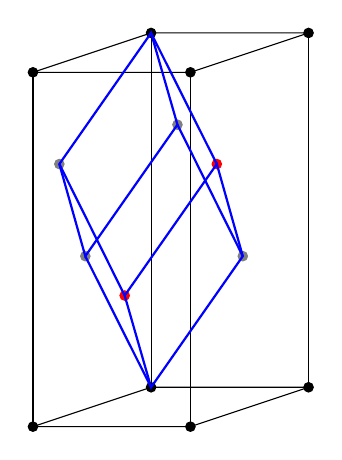
\begin{tikzpicture}[scale=0.5]
\coordinate (O)  at (0,0);
\coordinate (A)  at (4,0);
\coordinate (B)  at (7,1);
\coordinate (C)  at (3,1);
\coordinate (O1) at (0,9);
\coordinate (A1) at (4,9);
\coordinate (B1) at (7,10);
\coordinate (C1) at (3,10);
\draw (O)--(A)--(B)--(C)--cycle;
\draw (O1)--(A1)--(B1)--(C1)--cycle;
\draw (O)--(O1);
\draw (A)--(A1);
\draw (B)--(B1);
\draw (C)--(C1);

\coordinate (R1) at (4.67,6.67);
\coordinate (R2) at (2.33,3.33);
\coordinate (R3) at (5.33,4.33);
\coordinate (R4) at (1.33,4.33);
\coordinate (R5) at (0.67,6.67);
\coordinate (R6) at (3.67,7.67);


\foreach \p in {O,A,B,C,O1,A1,B1,C1}
{
    \filldraw (\p) circle (0.12);
}
\foreach \p in {R3,R4,R5,R6}
{
    \filldraw[gray] (\p) circle (0.12);
}
\foreach \p in {R1,R2}
{
    \filldraw[red] (\p) circle (0.12);
}
\draw[blue,thick] (C) -- (R2) -- (R1) -- (R3) --cycle;
\draw[blue,thick] (C1) -- (R6) -- (R4) -- (R5) --cycle;
\draw[blue,thick] (C) -- (R4);
\draw[blue,thick] (R1) -- (C1);
\draw[blue,thick] (R2) -- (R5);
\draw[blue,thick] (R3) -- (R6);
\end{tikzpicture}
\end{document}
    \end{figure}
    其中红色的点是R心六方晶胞内的点.记R心六方晶胞的三个边的向量为$\vec{a}$, $\vec{b}$和$\vec{c}$,菱方晶胞类似,则有
    \[\vec{a}'=\dfrac23\vec{a}+\dfrac13\vec{b}+\dfrac13\vec{c},\quad\vec{b}'=-\dfrac13\vec{a}+\dfrac13\vec{b}+\dfrac13\vec{c}\]
    于是
    \[a'=\sqrt{\vec{a}'\cdot\vec{a}'}=\sqrt{\dfrac49\vec{a}^2+\dfrac19\vec{b}^2+\dfrac19\vec{c}^2+\dfrac49\vec{a}\cdot\vec{b}}=\sqrt{\dfrac{1}{3}a^2+\dfrac19c^2}=\dfrac{\sqrt{3a^2+b^2}}{3}\]
    \[\cos\alpha'=\dfrac{\vec{a}'\cdot\vec{b}'}{a'b'}=\dfrac{-\dfrac{2}{9}\vec{a}^2+\dfrac19\vec{b}^2+\dfrac19\vec{a}\cdot\vec{b}+\dfrac19\vec{c}^2}{\dfrac{1}{3}a^2+\dfrac{1}{9}c^2}=\dfrac{-a^2+2c^2}{6a^2+2c^2}\]
    于是
    \[a'=\dfrac{\sqrt{3a^2+b^2}}{3},\quad\alpha=\arccos\left(\dfrac{-a^2+2c^2}{6a^2+2c^2}\right)\]
\end{solution}
\begin{homework}[7.]
    回答下面的问题.
    \begin{enumerate}[label=\tbf{(\alph*)}]
        \item 写出下图中用蓝色标记的平面的晶面指标及直角坐标系下的平面方程(记晶胞参数为$d$).
        \item 试在以下晶胞中找出符合指定晶面指标的三个晶面.
    \end{enumerate}
\end{homework}
\begin{solution}
    \begin{enumerate}[label=\tbf{(\alph*)}]
        \item \begin{enumerate}[label=\tbf{(\roman*)}]
            \item 晶面指标: $011$,平面方程: $y+z=d$.
            \item 晶面指标: $111$,平面方程: $x+y+z=d$.
        \end{enumerate}
        \item \begin{enumerate}[label=\tbf{(\roman*)}]
            \item 如下图所示:
            \begin{figure}[H]\centering
                \begin{subfigure}[b]{.3\linewidth}\centering
                    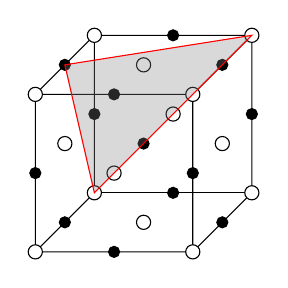
\begin{tikzpicture}[scale=0.5]
                        \draw[-] (0,0) -- (4,0) -- (4,4) -- (0,4) -- (0,0) -- (1.5,1.5) -- (1.5,5.5) -- (5.5,5.5) -- (5.5,1.5) -- (4,0);
                        \draw[-] (4,4) -- (5.5,5.5);
                        \draw[-] (0,4) -- (1.5,5.5);
                        \draw[-] (1.5,1.5) -- (5.5,1.5);
                        \filldraw[fill=white,draw=black] (0,0) circle (0.18);
                        \filldraw[fill=white,draw=black] (4,0) circle (0.18);
                        \filldraw[fill=white,draw=black] (4,4) circle (0.18);
                        \filldraw[fill=white,draw=black] (0,4) circle (0.18);
                        \filldraw[fill=white,draw=black] (1.5,1.5) circle (0.18);
                        \filldraw[fill=white,draw=black] (5.5,1.5) circle (0.18);
                        \filldraw[fill=white,draw=black] (5.5,5.5) circle (0.18);
                        \filldraw[fill=white,draw=black] (1.5,5.5) circle (0.18);
                        \filldraw[fill=white,draw=black] (2,2) circle (0.18);
                        \filldraw[fill=white,draw=black] (3.5,3.5) circle (0.18);
                        \filldraw[fill=white,draw=black] (0.75,2.75) circle (0.18);
                        \filldraw[fill=white,draw=black] (4.75,2.75) circle (0.18);
                        \filldraw[fill=white,draw=black] (2.75,0.75) circle (0.18);
                        \filldraw[fill=white,draw=black] (2.75,4.75) circle (0.18);

                        \filldraw[fill=black] (2,0) circle (0.14);
                        \filldraw[fill=black] (4.75,0.75) circle (0.14);
                        \filldraw[fill=black] (2,4) circle (0.14);
                        \filldraw[fill=black] (0.75,0.75) circle (0.14);
                        \filldraw[fill=black] (0,2) circle (0.14);
                        \filldraw[fill=black] (5.5,3.5) circle (0.14);
                        \filldraw[fill=black] (1.5,3.5) circle (0.14);
                        \filldraw[fill=black] (4,2) circle (0.14);
                        \filldraw[fill=black] (3.5,1.5) circle (0.14);
                        \filldraw[fill=black] (3.5,5.5) circle (0.14);
                        \filldraw[fill=black] (0.75,4.75) circle (0.14);
                        \filldraw[fill=black] (4.75,4.75) circle (0.14);
                        \filldraw[fill=black] (2.75,2.75) circle (0.14);
                        \filldraw[
                            fill = gray,
                            fill opacity = 0.3,
                            draw = red
                        ]
                        (0.75,4.75) -- (5.5,5.5) --(1.5,1.5) --cycle;
                    \end{tikzpicture}
                \end{subfigure}
                \begin{subfigure}[b]{.3\linewidth}\centering
                    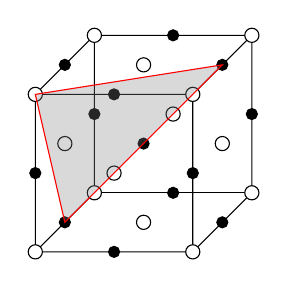
\begin{tikzpicture}[scale=0.5]
                        \draw[-] (0,0) -- (4,0) -- (4,4) -- (0,4) -- (0,0) -- (1.5,1.5) -- (1.5,5.5) -- (5.5,5.5) -- (5.5,1.5) -- (4,0);
                        \draw[-] (4,4) -- (5.5,5.5);
                        \draw[-] (0,4) -- (1.5,5.5);
                        \draw[-] (1.5,1.5) -- (5.5,1.5);
                        \filldraw[fill=white,draw=black] (0,0) circle (0.18);
                        \filldraw[fill=white,draw=black] (4,0) circle (0.18);
                        \filldraw[fill=white,draw=black] (4,4) circle (0.18);
                        \filldraw[fill=white,draw=black] (0,4) circle (0.18);
                        \filldraw[fill=white,draw=black] (1.5,1.5) circle (0.18);
                        \filldraw[fill=white,draw=black] (5.5,1.5) circle (0.18);
                        \filldraw[fill=white,draw=black] (5.5,5.5) circle (0.18);
                        \filldraw[fill=white,draw=black] (1.5,5.5) circle (0.18);
                        \filldraw[fill=white,draw=black] (2,2) circle (0.18);
                        \filldraw[fill=white,draw=black] (3.5,3.5) circle (0.18);
                        \filldraw[fill=white,draw=black] (0.75,2.75) circle (0.18);
                        \filldraw[fill=white,draw=black] (4.75,2.75) circle (0.18);
                        \filldraw[fill=white,draw=black] (2.75,0.75) circle (0.18);
                        \filldraw[fill=white,draw=black] (2.75,4.75) circle (0.18);

                        \filldraw[fill=black] (2,0) circle (0.14);
                        \filldraw[fill=black] (4.75,0.75) circle (0.14);
                        \filldraw[fill=black] (2,4) circle (0.14);
                        \filldraw[fill=black] (0.75,0.75) circle (0.14);
                        \filldraw[fill=black] (0,2) circle (0.14);
                        \filldraw[fill=black] (5.5,3.5) circle (0.14);
                        \filldraw[fill=black] (1.5,3.5) circle (0.14);
                        \filldraw[fill=black] (4,2) circle (0.14);
                        \filldraw[fill=black] (3.5,1.5) circle (0.14);
                        \filldraw[fill=black] (3.5,5.5) circle (0.14);
                        \filldraw[fill=black] (0.75,4.75) circle (0.14);
                        \filldraw[fill=black] (4.75,4.75) circle (0.14);
                        \filldraw[fill=black] (2.75,2.75) circle (0.14);
                        \filldraw[
                            fill = gray,
                            fill opacity = 0.3,
                            draw = red
                        ]
                        (0,4) -- (4.75,4.75) --(0.75,0.75) --cycle;
                    \end{tikzpicture}
                \end{subfigure}
                \begin{subfigure}[b]{.3\linewidth}\centering
                    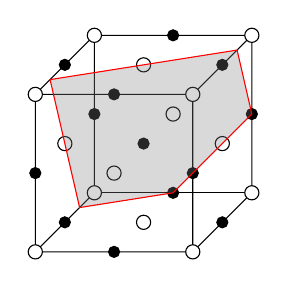
\begin{tikzpicture}[scale=0.5]
                        \draw[-] (0,0) -- (4,0) -- (4,4) -- (0,4) -- (0,0) -- (1.5,1.5) -- (1.5,5.5) -- (5.5,5.5) -- (5.5,1.5) -- (4,0);
                        \draw[-] (4,4) -- (5.5,5.5);
                        \draw[-] (0,4) -- (1.5,5.5);
                        \draw[-] (1.5,1.5) -- (5.5,1.5);
                        \filldraw[fill=white,draw=black] (0,0) circle (0.18);
                        \filldraw[fill=white,draw=black] (4,0) circle (0.18);
                        \filldraw[fill=white,draw=black] (4,4) circle (0.18);
                        \filldraw[fill=white,draw=black] (0,4) circle (0.18);
                        \filldraw[fill=white,draw=black] (1.5,1.5) circle (0.18);
                        \filldraw[fill=white,draw=black] (5.5,1.5) circle (0.18);
                        \filldraw[fill=white,draw=black] (5.5,5.5) circle (0.18);
                        \filldraw[fill=white,draw=black] (1.5,5.5) circle (0.18);
                        \filldraw[fill=white,draw=black] (2,2) circle (0.18);
                        \filldraw[fill=white,draw=black] (3.5,3.5) circle (0.18);
                        \filldraw[fill=white,draw=black] (0.75,2.75) circle (0.18);
                        \filldraw[fill=white,draw=black] (4.75,2.75) circle (0.18);
                        \filldraw[fill=white,draw=black] (2.75,0.75) circle (0.18);
                        \filldraw[fill=white,draw=black] (2.75,4.75) circle (0.18);

                        \filldraw[fill=black] (2,0) circle (0.14);
                        \filldraw[fill=black] (4.75,0.75) circle (0.14);
                        \filldraw[fill=black] (2,4) circle (0.14);
                        \filldraw[fill=black] (0.75,0.75) circle (0.14);
                        \filldraw[fill=black] (0,2) circle (0.14);
                        \filldraw[fill=black] (5.5,3.5) circle (0.14);
                        \filldraw[fill=black] (1.5,3.5) circle (0.14);
                        \filldraw[fill=black] (4,2) circle (0.14);
                        \filldraw[fill=black] (3.5,1.5) circle (0.14);
                        \filldraw[fill=black] (3.5,5.5) circle (0.14);
                        \filldraw[fill=black] (0.75,4.75) circle (0.14);
                        \filldraw[fill=black] (4.75,4.75) circle (0.14);
                        \filldraw[fill=black] (2.75,2.75) circle (0.14);
                        \filldraw[
                            fill = gray,
                            fill opacity = 0.3,
                            draw = red
                        ]
                        (0.375,4.375) -- (1.125,1.125) -- (3.5,1.5) -- (5.5,3.5) -- (5.125,5.125) --cycle;
                    \end{tikzpicture}
                \end{subfigure}
            \end{figure}
            \item 如下图所示:\begin{figure}[H]
                \centering\includegraphics[scale=0.15]{figure/7.png}
            \end{figure}
            分别过同一平面内的~\ce{H}原子,~\ce{O}原子和~\ce{Co}原子.
        \end{enumerate}
    \end{enumerate}
\end{solution}
\begin{homework}[8]
    试在以下点阵中画出符合指定晶面指标的三个平行晶面: $(100)$, $(210)$, $(1\bar{2}0)$ ,$(\bar{2}10)$, $(230)$ ,$(010)$.
\end{homework}
\begin{solution}
    如下图所示.
    \begin{figure}[H]\centering
        \begin{subfigure}[b]{.3\linewidth}\centering
            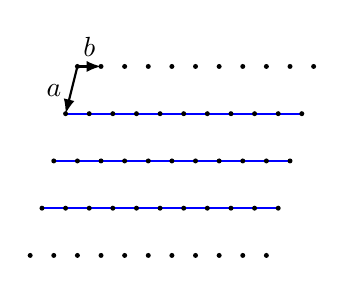
\begin{tikzpicture}[scale=0.3]
            \def\ax{-0.5}
            \def\ay{-2}
            \def\bx{1}
            \def\by{0}
            \draw[thick,blue] (\ax,\ay)--({\ax+10*\bx},\ay);
            \draw[thick,blue] ({2*\ax},{2*\ay})--({2*\ax+10*\bx},{2*\ay});
            \draw[thick,blue] ({3*\ax},{3*\ay})--({3*\ax+10*\bx},{3*\ay});
            \foreach \j in {0,...,10}
            {\foreach \i in {0,...,4}
                {\fill ({\i*\ax+\j*\bx},
                        {\i*\ay+\j*\by}) circle (3pt);}}
            \draw[thick,-latex]
                (0,0)--(\ax,\ay)
                node[midway,left] {$a$};
            \draw[thick,-latex]
                (0,0)--(\bx,\by)
                node[midway,above] {$b$};
            \end{tikzpicture}
            \caption{$100$}
        \end{subfigure}
        \begin{subfigure}[b]{.3\linewidth}\centering
            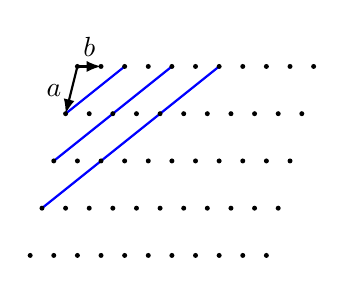
\begin{tikzpicture}[scale=0.3]
            \def\ax{-0.5}
            \def\ay{-2}
            \def\bx{1}
            \def\by{0}
            \draw[thick,blue] ({\ax},{\ay})--({2*\bx},{2*\by});
            \draw[thick,blue] ({2*\ax},{2*\ay})--({4*\bx},{4*\by});
            \draw[thick,blue] ({3*\ax},{3*\ay})--({6*\bx},{6*\by});
            \foreach \j in {0,...,10}
            {\foreach \i in {0,...,4}
                {\fill ({\i*\ax+\j*\bx},
                        {\i*\ay+\j*\by}) circle (3pt);}}
            \draw[thick,-latex]
                (0,0)--(\ax,\ay)
                node[midway,left] {$a$};
            \draw[thick,-latex]
                (0,0)--(\bx,\by)
                node[midway,above] {$b$};
            \end{tikzpicture}
            \caption{$210$}
        \end{subfigure}
        \begin{subfigure}[b]{.3\linewidth}\centering
            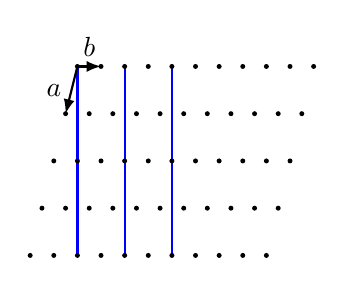
\begin{tikzpicture}[scale=0.3]
            \def\ax{-0.5}
            \def\ay{-2}
            \def\bx{1}
            \def\by{0}
            \draw[thick,blue] ({0*\bx},{0})--({4*\ax+2*\bx},{4*\ay});
            \draw[thick,blue] ({2*\bx},{0})--({4*\ax+4*\bx},{4*\ay});
            \draw[thick,blue] ({4*\bx},{0})--({4*\ax+6*\bx},{4*\ay});
            \foreach \j in {0,...,10}
            {\foreach \i in {0,...,4}
                {\fill ({\i*\ax+\j*\bx},
                        {\i*\ay+\j*\by}) circle (3pt);}}
            \draw[thick,-latex]
                (0,0)--(\ax,\ay)
                node[midway,left] {$a$};
            \draw[thick,-latex]
                (0,0)--(\bx,\by)
                node[midway,above] {$b$};
            \end{tikzpicture}
            \caption{$1\bar{2}0$}
        \end{subfigure}
        \begin{subfigure}[b]{.3\linewidth}\centering
            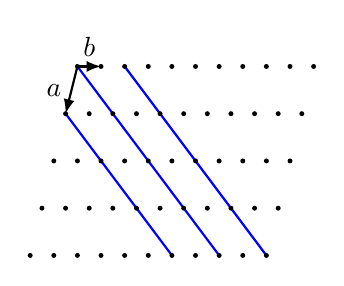
\begin{tikzpicture}[scale=0.3]
            \def\ax{-0.5}
            \def\ay{-2}
            \def\bx{1}
            \def\by{0}
            \draw[thick,blue] ({0*\bx},{0})--({4*\ax+8*\bx},{4*\ay});
            \draw[thick,blue] ({2*\bx},{0})--({4*\ax+10*\bx},{4*\ay});
            \draw[thick,blue] ({\ax},{\ay})--({4*\ax+6*\bx},{4*\ay});
            \foreach \j in {0,...,10}
            {\foreach \i in {0,...,4}
                {\fill ({\i*\ax+\j*\bx},
                        {\i*\ay+\j*\by}) circle (3pt);}}
            \draw[thick,-latex]
                (0,0)--(\ax,\ay)
                node[midway,left] {$a$};
            \draw[thick,-latex]
                (0,0)--(\bx,\by)
                node[midway,above] {$b$};
            \end{tikzpicture}
            \caption{$\bar{2}10$}
        \end{subfigure}
        \begin{subfigure}[b]{.3\linewidth}\centering
            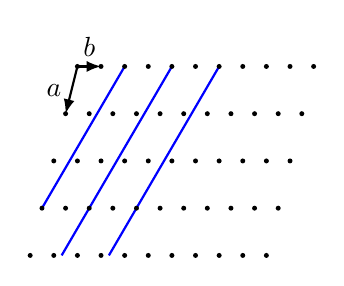
\begin{tikzpicture}[scale=0.3]
            \def\ax{-0.5}
            \def\ay{-2}
            \def\bx{1}
            \def\by{0}
            \draw[thick,blue] ({3*\ax},{3*\ay})--({2*\bx},{2*\by});
            \draw[thick,blue] ({4*\ax + 1.333*\bx},{4*\ay + 1.333*\by})--({4*\bx},{4*\by});
            \draw[thick,blue] ({4*\ax + 3.333*\bx},{4*\ay + 3.333*\by})--({6*\bx},{6*\by});
            \foreach \j in {0,...,10}
            {\foreach \i in {0,...,4}
                {\fill ({\i*\ax+\j*\bx},
                        {\i*\ay+\j*\by}) circle (3pt);}}
            \draw[thick,-latex]
                (0,0)--(\ax,\ay)
                node[midway,left] {$a$};
            \draw[thick,-latex]
                (0,0)--(\bx,\by)
                node[midway,above] {$b$};
            \end{tikzpicture}
            \caption{$230$}
        \end{subfigure}
        \begin{subfigure}[b]{.3\linewidth}\centering
            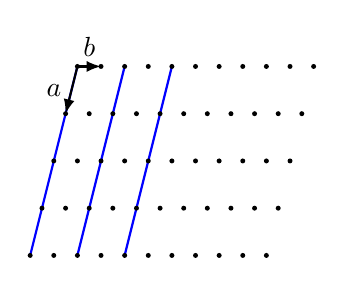
\begin{tikzpicture}[scale=0.3]
            \def\ax{-0.5}
            \def\ay{-2}
            \def\bx{1}
            \def\by{0}
            \draw[thick,blue] ({0*\bx+0*\ax},{0*\ay})--({0*\bx+4*\ax},{4*\ay});
            \draw[thick,blue] ({2*\bx+0*\ax},{0*\ay})--({2*\bx+4*\ax},{4*\ay});
            \draw[thick,blue] ({4*\bx+0*\ax},{0*\ay})--({4*\bx+4*\ax},{4*\ay});
            \foreach \j in {0,...,10}
            {\foreach \i in {0,...,4}
                {\fill ({\i*\ax+\j*\bx},
                        {\i*\ay+\j*\by}) circle (3pt);}}
            \draw[thick,-latex]
                (0,0)--(\ax,\ay)
                node[midway,left] {$a$};
            \draw[thick,-latex]
                (0,0)--(\bx,\by)
                node[midway,above] {$b$};
            \end{tikzpicture}
            \caption{$010$}
        \end{subfigure}
    \end{figure}
\end{solution}
\begin{homework}[9.]
    回答下面的问题.
    \begin{enumerate}[label=\tbf{(\alph*)}]
        \item 任何三维晶胞都可以取做平行六面体.记晶格矢量为$\vec{a}$, $\vec{b}$和$\vec{c}$,试证明晶胞体积$V=\left|\vec{a}\cdot(\vec{b}\times\vec{c})\right|$.
        \item 试证明三斜晶胞的体积为
        \[V=abc\sqrt{1-\cos^2\alpha-\cos^2\beta-\cos^2\gamma+2\cos\alpha\cos\beta\cos\gamma}\]
        \item 已知二水合草酸属于单斜晶系,晶胞参数$a=\SI{609.68}{\pico\meter}$, $b=\SI{349.75}{\pico\meter}$, $c=\SI{1194.6}{\pico\meter}$, $\beta=105.78^\circ$,密度$\rho=\SI{1.65}{\gram\per\centi\meter^3}$.试计算每个晶胞中二水合草酸的个数.
        \item 已知已知~\ce{Rb3TlF6}属于四方晶系,晶胞参数$a=\SI{651}{\pico\meter}$, $c=\SI{934}{\pico\meter}$,密度$\rho=\SI{4.45}{\gram\per\centi\meter^3}$.试计算每个晶胞中~\ce{Rb3TlF6}的数目.
        \item 试计算以下晶体的密度:\begin{enumerate}[label=\tbf{(\roman*)}]
            \item 金刚石:~\ce{C-C}键长为$\SI{154.5}{\pico\meter}$.
            \item 石墨:~\ce{C-C}键长为$\SI{142.0}{\pico\meter}$,层间距为$\SI{339.5}{\pico\meter}$.
        \end{enumerate}
    \end{enumerate}
\end{homework}
\begin{solution}
    \begin{enumerate}[label=\tbf{(\alph*)}]
        \item 考虑平行六面体以$\vec{b}$与$\vec{c}$张成的面作为底.于是其高为$\vec{a}$垂直于该平面的投影长度,即在$\vec{b}\times\vec{c}$上的投影长度,即
        \[h=\dfrac{\left|\vec{a}\cdot\left(\vec{b}\times\vec{c}\right)\right|}{\left|\vec{b}\times\vec{c}\right|}\]
        而底面的面积为
        \[S=bc\sin\theta=\left|\vec{b}\times\vec{c}\right|\]
        于是体积为
        \[V=Sh=\dfrac{\left|\vec{a}\cdot\left(\vec{b}\times\vec{c}\right)\right|}{\left|\vec{b}\times\vec{c}\right|}\left|\vec{b}\times\vec{c}\right|=\left|\vec{a}\cdot(\vec{b}\times\vec{c})\right|\]
        \item 首先
        \[V^2=\left|\vec{a}\cdot(\vec{b}\times\vec{c})\right|^2=\begin{vmatrix}
            \vec{a}\cdot\vec{a}&\vec{a}\cdot\vec{b}&\vec{a}\cdot\vec{c}\\
            \vec{b}\cdot\vec{a}&\vec{b}\cdot\vec{b}&\vec{b}\cdot\vec{c}\\
            \vec{c}\cdot\vec{a}&\vec{c}\cdot\vec{b}&\vec{c}\cdot\vec{c}
        \end{vmatrix}\]
        而
        \[\vec{a}\cdot\vec{a}=a^2,\quad\vec{b}\cdot\vec{b}=b^2,\quad\vec{c}\cdot\vec{c}=c^2\]
        \[\vec{a}\cdot\vec{b}=ab\cos\gamma,\quad\vec{b}\cdot\vec{c}=bc\cos\alpha,\quad\vec{c}\cdot\vec{a}=ca\cos\beta\]
        于是
        \[V=\begin{vmatrix}
            a^2&ab\cos\gamma&ca\cos\beta\\
            ab\cos\gamma&b^2&bc\cos\alpha\\
            ca\cos\beta&bc\cos\alpha&c^2
        \end{vmatrix}=a^2b^2c^2(1-\cos^2\alpha-\cos^2\beta-\cos^2\gamma+2\cos\alpha\cos\beta\cos\gamma)\]
        于是
        \[V=abc\sqrt{1-\cos^2\alpha-\cos^2\beta-\cos^2\gamma+2\cos\alpha\cos\beta\cos\gamma}\]
        证毕.
        \item 由题意可得
        \[\begin{aligned}
            Z
            &=\dfrac{\rho N_{\text{A}}V}{M}\\
            &=\dfrac{\SI{1.65}{\gram\per\centi\meter^3}\cdot\SI{6.022e23}{\per\mole}\cdot(609.68\cdot349.75\cdot1194.6\cdot\sin105.78^\circ)\si{\pico\meter^3}}{(12.01\cdot2+1.008\cdot2+16.00\cdot4+18.016\cdot2)\si{\gram\per\mol}}\\
            &=\dfrac{\SI{243.57}{\gram\per\mole}}{\SI{126.07}{\gram\per\mole}}\\
            &\approx2
        \end{aligned}\]
        即一个晶胞内有$2$个二水合草酸.
        \item 由题意可得
        \[\begin{aligned}
            Z
            &=\dfrac{\rho N_{\text{A}}V}{M}\\
            &=\dfrac{\SI{4.45}{\gram\per\centi\meter^3}\cdot\SI{6.022e23}{\per\mole}\cdot(651^2\cdot934)\si{\pico\meter^3}}{(85.47\cdot3+204.38+19.00\cdot6)\si{\gram\per\mol}}\\
            &=\dfrac{\SI{1060.7}{\gram\per\mole}}{\SI{574.8}{\gram\per\mole}}\\
            &\approx2
        \end{aligned}\]
        即一个晶胞内有$2$个~\ce{Rb3TlF6}.
        \item \begin{enumerate}[label=\tbf{(\roman*)}]
            \item 首先
            \[a=\dfrac{4r(\ce{C}-\ce{C})}{\sqrt{3}}=\SI{356.8}{\pico\meter}\]
            于是
            \[\rho_{\text{金刚石}}=\dfrac{ZM}{N_{\text{A}}V}=\dfrac{8\cdot\SI{12.01}{\gram\per\mole}}{\SI{6.022e23}{\per\mole}(356.8^3)\si{\pico\meter^3}}=\SI{3.512}{\gram\per\centi\meter^3}\]
            \item 首先
            \[a=\sqrt{3}r(\ce{C-C})=\SI{245.9}{\pico\meter},\quad c=2d=\SI{679.0}{\pico\meter}\]
            于是
            \[\rho_{\text{石墨}}=\dfrac{ZM}{N_{\text{A}}V}=\dfrac{4\cdot\SI{12.01}{\gram\per\mole}}{\SI{6.022e23}{\per\mole}\left(245.9^2\cdot679.0\cdot\dfrac{\sqrt3}{2}\right)\si{\pico\meter^3}}=\SI{2.243}{\gram\per\centi\meter^3}\]
        \end{enumerate}
    \end{enumerate}
\end{solution}
\begin{homework}[10.]
    证明边长为$a$, $b$, $c$的正交晶体中$(hkl)$晶面的间距$d$可以由
    \[\dfrac{1}{d^2}=\dfrac{h^2}{a^2}+\dfrac{k^2}{b^2}+\dfrac{l^2}{c^2}\]
    给出.
\end{homework}
\begin{proof}
    这一晶面过$\left(\dfrac{a}{h},0,0\right)$, $\left(0,\dfrac{b}{k},0\right)$和$\left(0,0,\dfrac{c}{l}\right)$.设平面的法向量为$\vec{n}$,则有
    \[\left(\dfrac{a}{h},-\dfrac{b}{k},0\right)\cdot\vec{n}=0,\quad\left(\dfrac{a}{h},0,-\dfrac{c}{l}\right)\cdot\vec{n}=0\]
    解得
    \[\vec{n}=\left(\dfrac{h}{a},\dfrac{k}{b},\dfrac{l}{c}\right)\]
    晶面间距即原点到晶面的距离$d$即原点到晶面上任意点构成的向量在$\vec{n}$上的投影长度.因此,不妨取晶面上的点$\left(\dfrac{a}{h},0,0\right)$,则有
    \[d=\dfrac{\left(\dfrac{a}{h},0,0\right)\cdot\vec{n}}{|\vec{n}|}=\dfrac{1}{\sqrt{\dfrac{h^2}{a^2}+\dfrac{k^2}{b^2}+\dfrac{l^2}{c^2}}}\]
    于是
    \[\dfrac{1}{d^2}=\dfrac{h^2}{a^2}+\dfrac{k^2}{b^2}+\dfrac{l^2}{c^2}\]
\end{proof}
\begin{homework}[11.]
    已知金红石属于四方晶系,晶胞参数$a=\SI{458}{\pico\meter}$, $c=\SI{298}{\pico\meter}$,原子的分数坐标为
    \[\ce{Ti}:\,(0,0,0),\,(1/2,1/2,1/2)\]
    \[\ce{O}:\,(0.31,0.31,0),\,(0.69,0.69,0.69),\,(0.81,0.19,1/2),\,(0.19,0.81,1/2)\]
    试计算~\ce{Ti-O}键长.
\end{homework}
\begin{solution}
    晶体中存在两种~\ce{Ti-O}键长,分别为
    \[r_1=\sqrt{(0.31a)^2+(0.31a)^2}=\SI{201}{\pico\meter}\]
    \[r_2=\sqrt{(0.19a)^2+(0.19a)^2+(0.5c)^2}=\SI{193}{\pico\meter}\]
\end{solution}
\begin{homework}[12.]
    \ce{CaS}晶体具有~\ce{NaCl}结构,晶体密度为$\SI{2.581}{\gram\per\centi\meter^3}$.试回答以下问题:
    \begin{enumerate}[label=\tbf{(\alph*)}]
        \item 试分析以下指标的衍射线中哪些是允许的: 100, 110, 111, 200, 210, 211, 220, 222.
        \item 计算~\ce{Cu\ K}$\alpha$辐射$(\lambda=\SI{154.2}{\pico\meter})$的最小可观测Bragg角.
    \end{enumerate}
\end{homework}
\begin{solution}
    \begin{enumerate}[label=\tbf{(\alph*)}]
        \item ~\ce{NaCl}结构是cF点阵,当$h$, $k$和$l$指标同时有奇数和偶数时即发生消光.因此允许的指标为:\begin{center}
            111, 200, 220, 222
        \end{center}
        \item 首先计算晶胞参数.有
        \[a=\sqrt[3]{V}=\sqrt[3]{\dfrac{ZM}{N_{\text{A}}\rho}}=\sqrt[3]{\dfrac{4\cdot(40.08+32.07)\si{\per\mole}}{\SI{2.581}{\gram\per\centi\meter^3}\cdot\SI{6.0221e23}{\per\mole}}}=\SI{570.5}{\pico\meter}\]
        最小可观测Bragg角对应最小的晶面间距,即$h^2+k^2+l^2$最小的指标,对于~\ce{CaS}即$111$.于是
        \[\sin\theta=\dfrac{\lambda}{2a}\sqrt{h^2+k^2+l^2}=0.2341\]
        于是
        \[\theta=13.54^\circ\]
    \end{enumerate}
\end{solution}
\begin{homework}[13.]
    某~\ce{MO}型金属氧化物属于立方晶系,晶体密度为$\SI{3.581}{\gram\per\centi\meter^3}$.用X射线粉末法(\ce{Cu\ K}$\alpha$线)测得各衍射线相应的衍射角分别为
    \[18.5^\circ,\,21.5^\circ,\,31.2^\circ,\,37.4^\circ,\,39.4^\circ,\,47.1^\circ,\,52.9^\circ,\,54.9^\circ\]
    据此回答下面的问题:
    \begin{enumerate}[label=\tbf{(\alph*)}]
        \item 确定该金属氧化物晶体的点阵型式.
        \item 计算晶胞参数和一个晶胞中的结构基元数.
        \item 计算金属原子M的相对原子质量,说明M是什么元素.
    \end{enumerate}
\end{homework}
\begin{solution}
    \begin{enumerate}[label=\tbf{(\alph*)}]
        \item 以$18.5^\circ$对应的衍射线的指标$\sqrt{h_0^2+k_0^2+l_0^2}$作为基准,列出下表:
        \begin{table}[H]\centering
            \begin{tabular}{|c|c|c|c|c|c|c|c|c|}\hline
               $\theta$ & $18.5^\circ$ & $21.5^\circ$ & $31.2^\circ$ & $37.4^\circ$ & $39.4^\circ$ & $47.1^\circ$ & $52.9^\circ$ & $54.9^\circ$ \\\hline
               $\sin\theta$ & $0.317$ & $0.366$ & $0.518$ & $0.607$ & $0.634$ & $0.732$ & $0.798$ & $0.818$ \\\hline
               $\dfrac{h^2+k^2+l^2}{h_0^2+k_0^2+l_0^2}$ & $1$ & $1.33$ & $2.66$ & $3.66$ & $4.00$ & $5.33$ & $6.32$ & $6.65$\\\hline
            \end{tabular}
        \end{table}
        由此不难看出$h_0^2+k_0^2+l_0^2=3$,即$h_0=k_0=l_0=1$.所有衍射线的指标依次为
        \begin{center}
            111, 200, 220, 311, 222, 400, 331, 420
        \end{center}
        可以看出三个指标的奇偶性一致,因此该金属氧化物为cF点阵.
        \item 晶胞参数为
        \[a=\dfrac{\sqrt{h^2+k^2+l^2}\lambda}{2\sin\theta}\]
        取第一组数据可得
        \[a=\SI{420.9}{\pico\meter}\]
        由于该晶体属于cF点阵,因此晶胞内的结构基元数目为$4$.
        \item 一个结构基元的分子量为
        \[M=\dfrac{\rho N_{\text{A}}V}{Z}=\dfrac{\SI{3.581}{\gram\per\centi\meter^3}\cdot\SI{6.0221e23}{\per\mole}\cdot(420.9^3)\si{\pico\meter^3}}{4}=\SI{40.2}{\gram\per\mole}\]
        因此M的原子量为
        \[M_{\ce{M}}=M-M_{\ce{O}}=\SI{24.2}{\gram\per\mole}\]
        于是M为~\ce{Mg}.
    \end{enumerate}
\end{solution}
\end{document}